\documentclass[a4paper,twoside,11pt,pdftex,fleqn]{book}

%%%%%%%%%%%%%%%%%%%%%%%%%%%%%%%%%%%%%%%%%%%%%%%
%                  packages
%%%%%%%%%%%%%%%%%%%%%%%%%%%%%%%%%%%%%%%%%%%%%%%
\usepackage[T1]{fontenc}        % accents
%\usepackage{lmodern}
\usepackage[Lenny]{fncychap}    % en tete de chapitre
\usepackage[vscale=0.75,hscale=0.75,hmarginratio=5:4,vmarginratio=1:1,marginparsep=5pt,marginparwidth=2cm,headheight=15pt]{geometry} % layout
\usepackage{graphicx}                          % graphiques, images
\usepackage{amsmath,bbm,amssymb}               % math
%\usepackage[tight,hang,raggedright]{subfigure} % subfigures
\usepackage[tight]{subfigure} % subfigures
\usepackage{xspace}             % esapce a la fin des macros
\usepackage{fancyhdr}           % remplacement de tag postscript
\usepackage{icomma,hhline}      % virgule pour nombre reel
\usepackage{longtable}
\usepackage{makerobust}
\usepackage{algorithm,algorithmic}
%\usepackage{titlesec}
\usepackage{ifthen}
\usepackage{tabularx,caption}
\usepackage[square,sort&compress,numbers]{natbib}
\usepackage{pdfpages}
\usepackage[pagebackref=true,final,colorlinks=true]{hyperref} % hyperlinks
\usepackage{todonotes}

\graphicspath{{./FIGS/}} % Specifies the directory where pictures are stored


% MY PACKAGES
\usepackage{algorithm, algorithmic}

\begin{document}

\newcommand{\ra}[1]{\renewcommand{\arraystretch}{#1}}

% # Flow around contra-rotating open rotors: general information
%     * Background
%     * Aerodynamic of an isolated propeller
%     * Aerodynamic of a contra-rotating open rotor
%     * A few words on aeroelasticity
%         - experimental aeroelasticity
%         - numerical aeroelasticity
% 
% # Generalities
%     * equation that I solve
%     * elsA
%     * ALE / aeroelasticity presentation
%!TEX root = ../main.tex
\chapter{Generalities}
\label{generalities}

\lhead{Chapitre ??. \emph{Generalities}}

\section{Equation solved} % (fold)
\label{sec:equation_solved}

The Unsteady Reynolds-Averaged Navier-Stokes (U-RANS) equations in
integral form are given by
\begin{equation}
   \int_\Omega \frac{\partial W}{\partial t} dV + \oint_{\partial
     \Omega} \overrightarrow{F} \cdot \overrightarrow{N} ds = 0,
   \label{eq:intNS}
\end{equation} 
where $\overrightarrow{F}$~is the flux across $\partial \Omega$ and
$W$~is the vector of the conservative unknowns (conservative variables
and turbulent variables).  Assuming $\Omega$ is a
control volume, the semi-discrete finite-volume form of the
U-RANS equations is obtained from Eq.~\eqref{eq:intNS}:
\begin{equation}
   \frac{d}{dt} \left(V  \overline{W}\right) + R \left( \overline{W}
   \right) = 0,
   \label{eq:semiDiscNS}
\end{equation} 
with $V$~the volume of the cell~$\Omega$, $R$~the residual resulting
from the discretization of the fluxes and the source terms (including
the turbulent equations), and $\overline{W}$ the mean of the
unknowns over the control volume.  In the following, the over line
symbol~$\overline{\cdot}$ is dropped out for clarity.

\section{Fluid / Structure Interaction}

\subsection{Weak Coupling Approach}

The weak coupling approach~\cite{Rougeault2003} is a one way
  coupling from structure to fluid: First, a modal identification
of the structure is carried out. Then the fluid response to the
harmonic prescribed motion of the structure modes is simulated,
where the harmonic motion of the geometry is ensured by a mesh
deformation technique, based on a structural analogy method
implementing linear elastic elements. Finally, knowing the unsteady
pressure load, a stability study can be performed in the frequency
domain.

\subsection{Linear Modal Structure Model}

\subsubsection{Governing Equations}
Once the modal basis $\Phi$ is identified, either by mean of a Finite
Element model or an experimental identification, the equation of
structure dynamics under aerodynamic load $F_A$ reads:
\begin{equation}
  \label{eq:2}
  M\ddot{q}+D\dot{q}+Kq-\Phi^\top F_A(t)=0, \quad x=\Phi q.
\end{equation}
The weak coupling approach assumes the linearity of the response of
the fluid with respect to the displacement of the structure. Therefore
small displacements are assumed and the so-called Generalized
Aerodynamic Forces (GAF) are linearized, which adds aerodynamic
stiffness~$K_A$ and damping~$D_A$:
\begin{equation}
  \label{eq:4}
  \Phi^\top F_A(t) = D_A\dot{q}+K_Aq.
\end{equation}
In order to estimate the unsteady aerodynamic forces $F_A(t)$,
  a fluid simulation is run with a prescribed harmonic motion of the
  structure:
\begin{equation}
  \label{eq:6}
  q(t)=\cos(\omega t).
\end{equation}
A stability analysis is then performed in the frequency domain:
\begin{equation}
  \label{eq:5}
  q=\hat{q}e^{p t}\Rightarrow\left(
    p^2M + p(D-D_A) + (K-K_A)
  \right)\hat{q}=0,
\end{equation}
where the Laplace variable $p$ is of the form
$p=i\omega(1+i\alpha)$. Finally, considering only weakly damped or
amplified modes (i.e. $|\alpha| \ll 1$), the damping of the
fluid/structure coupled system reads $\alpha=-\Re e(p)/\Im m(p)$.

\subsubsection{Single Passage Reduction for Turbomachinery Computations}

As the blade row is rotating, the stiffness of the blades is increased
and gyroscopic terms are added. Equation~\eqref{eq:2} becomes
\begin{equation}
  \label{eq:gyr}
  M\ddot{q}+(D+D_G)\dot{q}+(K+K_G)q-\Phi^\top F_A(t)=0, \quad x=\Phi q,
\end{equation}
where $D_G$ is the skew-symmetric gyroscopic damping matrix and $K_G$ is
the gyroscopic matrix of deflection for inclusion of centrifugal
elements for instance.  The disk being flexible, the blades do not vibrate
independently of each other. The cyclic symmetry leads to complex
vibration modes, which can be seen as rotating waves traveling at an
integer multiple $n_d$ of the rotation speed \cite{Lane:1956fk}. $n_d$
is called a nodal diameter. Opposite nodal diameters have the same
vibration mode propagating in opposite directions. Therefore their
respective modes are complex conjugate.


% section aeroelasticity_module (end)

% section equation_solved (end)

% 
% # Harmonic balance methods
%     * state of the art
%         - Numeca
%         - Duke
%         - He
%     * mono-frequential
%         - theory
%         - advantages
%         - applications that can be treated
%!TEX root = ../main.tex
\chapter{Harmonic balance methods} % (fold)
\label{cha:harmonic_balance_methods}

\section{Periodic flows} % (fold)
\label{sec:periodic_flows}

If the mean flow variables $W$~are periodic in time of period $T =
2\pi/\omega$, so are the residuals $R(W)$ and the Fourier series of
Eq.~\eqref{eq:semiDiscNS} is
\begin{equation}
  \label{eq:seriefour}
  \sum_{k=-\infty}^\infty \left(ik\omega
    V\widehat{W}_k+\widehat{R}_k\right)e^{ik\omega t}=0,
\end{equation}
where $\widehat{W}_k$ and $\widehat{R}_k$ are the Fourier coefficients
of $W$ and $R$ corresponding to the mode~$k$:
\begin{equation}
   W(t) = \sum_{k=-\infty}^{\infty} \widehat{W}_k e^{i k\omega t},\quad
   R(t) = \sum_{k=-\infty}^{\infty} \widehat{R}_k e^{i k\omega t}.
   \label{eq:fourierWsf}
\end{equation}
The complex exponential family forming an orthogonal basis, the only
way for Eq.~\eqref{eq:seriefour} to be true is that the weight of
every mode $k$ is zero, which leads to an infinite number of steady
equations in the frequency domain:
\begin{equation}
  \label{eq:orthodelim}
  ik\omega V\widehat{W}_k+\widehat{R}_k=0, \quad \quad \forall k \in
  \mathbb{Z}.
\end{equation}
McMullen~\emph{et al.}~\cite{McMullen2001,McMullen2002,McMullen2006}
solve a subset of these equations up to mode~$N$, $-N\leq k\leq N$,
yielding the Non-Linear Frequency Domain (NLFD) method.

%As the present method has to be implemented in a time-domain solver,
%these equations are cast back into the time domain by mean of an
%Inverse Discrete Fourier Transform (IDFT) and the Time Spectral
%Method~(TSM)~\cite{Gopinath2005} is retrived.
The principle of the time-domain Harmonic Balance approach, sometimes
referred to as Time Spectral Method (TSM)~\cite{Gopinath2005,
  Sicot2008}, is to use an Inverse Discrete Fourier Transform (IDFT)
to cast the equations back into the time domain.  The IDFT then
induces linear relations between Fourier coefficients $\widehat{W}_k$
and a uniform sampling of $W$ at $2N+1$ instants in the period:
\begin{equation}
  W_n=\sum_{k=-N}^N\widehat{W}_k\exp(i\omega n\Delta t),\quad \quad 0 \leq n < 2N+1,
\end{equation}
with $W_n \equiv W(n \Delta t)$ and $\Delta t=T/(2N+1)$. This leads to
a new system of $2N+1$~mathematically steady equations coupled by a
source term:
\begin{equation}
  \label{eq:hbttime}
  R(W_n)+VD_t(W_n)=0, \quad \quad 0 \leq n < 2N+1.
\end{equation}
The source term $VD_t(W_n)$ appears as a high-order formulation of the
initial time derivative in Eq.~\eqref{eq:semiDiscNS}. This new time
operator connects all the time levels and can be expressed
analytically as
\begin{equation}
\label{eq:dt}
  D_t(W_n)=\sum_{m=-N}^{N} d_m W_{n+m},
\end{equation}
with
\begin{equation}
  d_m=
  \begin{cases}
    \frac{\pi}{T}(-1)^{m+1}\csc\left(\frac{\pi
        m}{2N+1}\right) &, \, m\neq 0,\\
    0 &, \, m=0.
  \end{cases}
\end{equation}
This equation clearly states that the source term is real for periodic flows.
A similar derivation can be made for an even number of instants, but
it is proved in Ref.~\cite{Weide2005} that it can lead to a numerically unstable odd-even
decoupling. % and as a consequence, the method can become
%unstable. % Time-dependent boundary conditions could also benefit from
% such a derivation, but this is not an issue for external aerodynamic
% applications and has not been done yet.

A pseudo-time ($\tau_n$) derivative is added to
Eqs.~\eqref{eq:hbttime} to march the equations in pseudo-time to the
steady-state solutions of all the instants:
\begin{equation}
  \label{eq:pseudohbttime}
  V\frac{\partial W_n}{\partial\tau_n} + R(W_n)+VD_t(W_n)=0, \quad \quad
  0 \leq n < 2N+1.
\end{equation}
This time step is defined locally in a given cell and can
  be different for all the HB instants. For stability reasons, its
computation is modified~\cite{Weide2005} to take into account
the additional source term,
\begin{equation}
  \label{eq:stabdeltat}
  \Delta\tau_n=\text{CFL}\frac{V}{\|\xi_n\|+\omega NV}.
\end{equation}
The extra term $\omega NV$ is added to the spectral radius $\|\xi_n\|$ to
restrict the time step.  Equation~\eqref{eq:stabdeltat} implies that a
high frequency and/or a high number of harmonics~$N$ can considerably
restrict the time step, especially for explicit Runge Kutta time
integration scheme, as mentioned in~\cite{Hall2002}. % Actually, it has been
% observed~\cite{Hall2002} that the convergence of the method slows down
% for increasing~$N$\todo{compacter}. All the cited references use
% explicit schemes, such as Runge-Kutta, to carry out the pseudo-time
% integration. Their limit stability criteria on CFL numbers is very
% sensitive to such a restriction.
%Conversely, implicit schemes are more
%stable and allow larger CFL numbers. 
Several implicit schemes, which are theoretically unconditionally stable and thus allow larger
CFL number, have been derived for the HB method: Krylov-space based
methods are used
in~\cite{FLD:FLD2111,woodgate09:_implic_harmon_balan_solver_for}, and
Antheaume~\emph{et
  al.}~\cite{antheaume11:_implic_time_spect_method_for} propose a
point Jacobi algorithm. The present paper uses the block-Jacobi
algorithm derived in Ref.~\cite{Sicot2008} to improve robustness and
efficiency.

This time-domain harmonic balance method has been implemented in the
\emph{elsA} solver~\cite{cambier2012} developed by ONERA and
CERFACS. This code solves the RANS equations using a cell-centered
approach on multi-blocks structured meshes.  Using the HB method, significant savings in
CPU cost have been observed in various applications such as dynamic
derivatives computation~\cite{Hassan2011},
aeroelasticity~\cite{Dufour2010} and rotor/stator
interactions~\cite{Sicot2012}. However, this approach is limited to
periodic flows (\emph{i.e.} a single fundamental frequency) and is
unfit when the main frequencies of the system are not integers multiple
of each other (such as multi-stage turbomachines for instance). The single-frequency HB method is therefore
extended to the case where the flow is not periodic in time but is
almost periodic.

\subsubsection{Adaptation to the ALE Formulation}
\label{sec:adapt-ale-form}

The deformation speed $s_D$ is estimated by applying the HB time
derivative operator to the mesh points at all instants:
$s_D^*=D_t(X^*)$. This decomposition is exact when the
  deformation of the mesh has less harmonics than those solved in the
  HB computation~\cite{Dufour2010}. In the present case, the mesh
  deformation follows a purely single frequency law (see
  Eq.~\eqref{eq:6}), therefore all the HB computations will correctly
  estimate the mesh deformation speed regardless of their harmonic content.


\subsubsection{Adaptation to Turbomachinery Single Passage
    Reduction}
\label{sec:Adptatreduction}

The phaselag periodic condition can be derived by applying an
  IDFT on the phase-shifted harmonics ($\widehat{W}_ke^{ik\beta}$) of
  Eq.~????. A linear
combination of all the time instants is obtained:
\begin{equation}
  % \label{eq:16}
  W^*\left(\theta+\phi\frac{2\pi}{B}\right)=\mathcal{E}^{-1}\mathcal{M}\mathcal{E}W^*(\theta),\quad \phi=\pm 1,
\end{equation}
where $\mathcal{M}$ is a diagonal matrix equal to the IBPA modulation
$\mathcal{M}_{k,k}=e^{i k\beta}$. It can be derived
analytically in the same way as the source term Eqs.~ ???
and~ ???:
\begin{equation}
  W\left(x, r, \theta+\phi\frac{2\pi}{B}, t_n\right) =\sum_{m=-N}^N
  b_mW(x, r, \theta, t_{n+m}), 
\end{equation}
%  and can be derived
% analytically in the same way as the source term Eqs.~\eqref{eq:hbtdt} and~\eqref{eq:3}:
% \begin{equation}
%   % \label{eq:16}
%   W^*\left(\theta+\phi\frac{2\pi}{B}\right)=\mathcal{E}^{-1}\mathcal{M}\mathcal{E}W^*(\theta)\
%   \Leftrightarrow\ 
%   W\left(x, r, \theta+\phi\frac{2\pi}{B}, t_n\right) =\sum_{m=-N}^N
%   b_mW(x, r, \theta, t_{n+m}),
% \end{equation}
with
\begin{equation}
  b_m=\frac{1}{2N+1}\left(1+2\sum\nolimits_{k=1}^N\cos\left[k\left(2\pi
        \frac{m}{2N+1}-\phi \beta\right)\right]\right),\quad \phi=\pm 1.
\end{equation}
As the HB method solves and stores simultaneously a uniform sampling
of the time period, it could be considered similar to Erdos' direct
store method. Actually, the method used here is closer to the shape
correction~\cite{He1990}, in a sense that the lag is
computed thanks to Fourier series.%~\cite{Sicot2009}.

\section{Numerical Applications}
For external-flow aeroelasticity, the HB approach has been thoroughly validated~\cite{Gopinath2005,Sicot2008,Woodgate2009,Dufour2010}, mostly for the AGARD test cases of Davis~\cite{Davis1982}. However, experimental data for turbomachinery aeroelasticity are more scarce: the Standard Aeroelastic Configurations experiments of Fransson~\textit{et al.}~\cite{Fransson:1999uq} are the reference in this respect, and have been widely used to validate different numerical approaches~\cite{Sbardella:2001fk,Duta:2002uq,Campobasso:2003fk,Cinnella2004,mcbean2005}. However, this is the first time these results are used to validate HB simulations. %
The presented applications are in increasing complexity.  The first
test case is a turbine stator (STCF~11), for which experimental results are available at both subsonic and transonic conditions.  %The second test case is the
%transonic configuration of the STCF~11. The latter shows non-linear
%effects, such as shock and separation bubble, that helps assessing the
%capability of the HB method to correctly captures such phenomena.
The second test case is an industrial fan configuration, proving the
robustness of the method for industrial requirements.

% section periodic_flows (end)

% chapter harmonic_balance_methods (end)
%     * multi-frequential (advantages and questions that it raises)
%         - theory
%         - advantages
%         - applications that can be treated
%!TEX root = ../main.tex

montrer l'essence des méthodes spectrales avec une equation toute simple

depuis les années 1990 on essaye d emodeliser les instationnarite en TBM:
methode des deterministic stress puis LUR et enfin les methodes harmoniques.

\chapter{Spectral methods} % (fold)
\label{cha:spectral_methods}

\section{Introduction} % (fold)
\label{sec:sm_introduction}
% section introduction (end)

\section{State of the art} % (fold)
\label{sec:sm_state_of_the_art}

There is a large variety of spectral methods that exists in the
literature. The most important will be presented in this section.
As the development of these approaches on the Navier-Stokes equations
can be tedious, the following will only concentrate on the simplest
nonlinear equation, the advection equation for the velocity
defined as:
\begin{equation}
	\frac{\partial u}{\partial t} + 
	u \frac{\partial u}{\partial x} = 
	0.
	\label{eq:sm_nonlinear_convection}
\end{equation}
This equation can be formulated in a conservative manner for simplicity:
\begin{equation}
	\frac{\partial u}{\partial t} + 
	\frac{\partial}{\partial x} \left( \frac{u^2}{2} \right) = 
	0.
	\label{eq:sm_nonlinear_convection_conservative}
\end{equation}

The reader is referred to the cited papers for a detailed description
of the following methods and in particular, their
development for the Navier-Stokes equations. 

In total four spectral methods are presented, 
the Linearized Unsteady Reynolds averaged
Navier-Stokes, the NonLinear Harmonic method, the NonLinear Frequency Domain
method and the Harmonic Balance method.  
These names are chosen here
for simplicity but the reader might find in the literature many more
appellations. When it is the case, an effort will be made to synthesize
these to give the reader a good overview of the type of spectral methods available. Moreover, special emphasis will be put on the harmonic
balance method as it is the approach used in this thesis.

\subsection{Linearized} % (fold)
\label{sub:sm_linearized_method}

TO FILL

% subsection sm_linearized_method (end)

\subsection{The NonLinear Harmonic method} % (fold)
\label{sub:sm_nonlinear_harmonic_method}

Originally developed by \citet{He1998} and \citet{Ning1998},
the 
NonLinear Harmonic method
relies on a decomposition of the conservative variables into a
time-averaged part plus an unsteady perturbation:
\begin{equation}
	u = \overline{u} + u^\prime,
	\label{eq:sm_nlh_decomposition}
\end{equation}
where $\overline{.}$ denotes the time-averaging operator and
$.^\prime$ the corresponding unsteady perturbation.
By injecting Eq.~\ref{eq:sm_nlh_decomposition} into
Eq.~\ref{eq:sm_nonlinear_convection_conservative}, one gets:
\begin{equation}
	\frac{\partial u^\prime}{\partial t} + 
	\frac{1}{2}\frac{\partial}{\partial x} \left[
	\overline{u}^2 + 2 \overline{u} u^\prime + u^\prime u^\prime \right] = 
	0.
	\label{eq:sm_nlh_step_1}
\end{equation}
The time-averaged equation can be obtained by time-averaging
equation~\ref{eq:sm_nlh_step_1}:
\begin{equation}
	(\overline{\ref{eq:sm_nlh_step_1}})
	\Leftrightarrow
	\frac{\partial}{\partial x}
	\left[\overline{u}^2 + 
	\overline{u^\prime u^\prime}\right] =
	0,
	\label{eq:sm_nlh_step_2}
\end{equation}
The term $\overline{u^\prime u^\prime}$
appears due to the non-linearities of the considered equation. It
is called the nonlinear stress terms 
(or the deterministic stress terms) as a reference to 
the Reynolds stress terms. 
The equations for the unsteady perturbations is then obtained by keeping
the first order terms of the unsteady equation~\ref{eq:sm_nlh_step_1}.
This means that the term $u^\prime u^\prime$ is neglected and leads
to:
\begin{equation}
	\frac{\partial u^\prime}{\partial t} + 
	\frac{\partial}{\partial x} \left[\overline{u} u^\prime \right] = 
	0.
\end{equation}

\paragraph{Mono-frequential formulation}
For now on, no assumption has been made neither on the velocity $u$,
nor on its time-averaged part and unsteady perturbation part.
Now, assuming that the velocity perturbation 
is periodic in time with period
$T=2 \pi / \omega$,
the unsteady fluctuations can be decomposed into 
a Fourier series:
\begin{equation}
	u^\prime = \sum_{k=-\infty \atop k \neq 0}^{\infty} 
	\widehat{u}_k e^{i \omega k t}.
	\label{eq:sm_nlh_decomposition_pert}
\end{equation}
Hence, since the complex exponentials forms 
an orthogonal basis, we have for all harmonics 
$-\infty \leq k \leq \infty, \; k \neq 0$:
\begin{equation}
	i \omega k \widehat{u}_k + 
	\frac{\partial}{\partial x} \left[ \overline{u} \widehat{u}_k\right] =
	0.
\end{equation}
One can notice that the time-averaged part has been removed from
the Fourier series through $k \neq 0$.
Each harmonic equation represents now a steady equation as no temporal
derivative is present anymore.

The term $\overline{u^\prime u^\prime}$ remains in the time-averaged
equation and needs to be computed. It can be 
directly worked out when the harmonics are known:
\begin{equation}
	\begin{split}
		u^\prime u^\prime &= 
		\left[
			\sum_{k=-\infty \atop k \neq 0}^{\infty} \widehat{u}_k e^{i \omega k t} 
		\right]
		\left[
			\sum_{k=-\infty \atop k \neq 0}^{\infty} \widehat{u}_k e^{i \omega k t} 
		\right] \\
		&= \sum_{k=-\infty \atop k \neq 0}^{\infty} (\widehat{u}_k)^2
		   e^{i 2 \omega k t} +
		   2 \sum_{j,k=-\infty \atop j \neq k \neq 0}^{\infty} 
		   \widehat{u}_k \widehat{u}_j e^{i \omega (j + k) t} \\
	\end{split}
\end{equation}
Thus,
\begin{equation}
	\begin{split}
		\overline{u^\prime u^\prime} &= 
		\frac{1}{T} \int_{t=0}^{T} \left[ 
			\sum_{k=-\infty \atop k \neq 0}^{\infty} (\widehat{u}_k)^2
		   	e^{i 2 \omega k t} +
		   	2 \sum_{j,k=-\infty \atop j \neq k \neq 0}^{\infty} 
		   	\widehat{u}_k \widehat{u}_j e^{i \omega (j + k) t} 
		\right] dt\\
		&= \frac{2}{T} \int_{t=0}^{T} \sum_{j,k=-\infty \atop j \neq k \neq 0}^{\infty} 
		   	\widehat{u}_k \widehat{u}_j 
		   	e^{i \omega (j + k) t} dt \\
		&= \frac{2}{T} \int_{t=0}^{T} 
			\sum_{k=-\infty \atop k \neq 0}^{\infty} 
			\widehat{u}_k \widehat{u}_{-k}  dt.
	\end{split}
\end{equation}
As $\widehat{u}_k$ and $\widehat{u}_{-k}$ are complex conjugates,
finally $\overline{u^\prime u^\prime}$ is equal to:
\begin{equation}
	\overline{u^\prime u^\prime} = 
	2 \sum_{k=-\infty \atop k \neq 0}^{\infty} |\widehat{u}_k|^2.
	\label{eq:sm_nlh_deterministic_stress_terms}
\end{equation}
This last equation only depends on the computed harmonics, meaning
that no term is modelled. Moreover, this term couple the
time-average with the unsteady perturbations. This is this
terms that is \todo{LUR}

Finally, as computing an infinite number of harmonics is not feasible,
the number of harmonics is truncated at order $N$. 
This is a fare assumption as most
of the physical flows have a finite unsteady spectrum. This
is for sure a reduce order approach. The goal of the spectral
methods being to have a compact representation of the unsteady time
signals. As for a mesh grid convergence, the number of harmonics $N$
is increased until the unsteady representation of the signal is
converged for the variable of interest. The discussion on the
convergence of spectral methods will be detailed later on in sec
\todo{section convergence}.


To summarize, the NonLinear Harmonic
method applied to Eq.~\ref{eq:sm_nonlinear_convection_conservative},
gives $2N + 1$ equations:
\begin{equation}
	\fbox{$
	\begin{cases}
		\displaystyle 
		\frac{\partial}{\partial x}
			\left[\overline{u}^2 + 
			\overline{u^\prime u^\prime}\right] &=
			0, \\
		\displaystyle
		i \omega k \widehat{u}_k + 
			\frac{\partial}{\partial x} 
			\left[ \overline{u} \widehat{u}_k\right] &= 
			0, \: k \in [-N, N], \: k \neq 0,
	\end{cases}
	$}
	\label{eq:sm_nlh_subset_eq}
\end{equation}
coupled by the deterministic stress term $\overline{u^\prime u^\prime}$
defined in Eq.~\ref{eq:sm_nlh_deterministic_stress_terms}.
Three hypothesis lies under these equations:
\begin{itemize}
	\item the unsteady perturbations are periodic in time
	with period $T= 2 \pi / \omega$, 
	meaning that they can be decomposed into a Fourier series,
	\item the high-order cross-coupling terms $u^\prime u^\prime$
	are neglected,
	\item the number of harmonics is set to $N$.
\end{itemize}

\paragraph{Multi-frequential formulation}

In \citet{He2002}, the method is extended to a multi-frequential
perturbation. Instead of writing them
using a Fourier series as defined in Eq.~\ref{eq:sm_nlh_decomposition_pert},
these are written using a sum of harmonics each of which
having a frequency $\omega_k$:
\begin{equation}
	u^\prime = \sum_{k=-N \atop k \neq 0}^{N} 
	\widehat{u}_k e^{i \omega_k t}.
	\label{eq:sm_nlh_decomposition_pert_multi}
\end{equation}
Note that the term $k \omega$ in Eq.~\ref{eq:sm_nlh_decomposition_pert}
is now $\omega_k$ meaning that frequencies can be chosen
arbitrarily. In the paper of \citet{He2002}, no mathematical
framework that allows this decomposition is given. To the author
knowledge, it is only in \cite{JGuedeney2013} that the mathematical
justifications that allows writing 
\ref{eq:sm_nlh_decomposition_pert_multi} are given.
The derivation of the equations are kept the same and the following
$2N+1$ subset of equations are given:
\begin{equation}
	\fbox{$
	\begin{cases}
		\displaystyle 
		\frac{\partial}{\partial x}
			\left[\overline{u}^2 + 
			\overline{u^\prime u^\prime}\right] &=
			0, \\
		\displaystyle
		i \omega_k \widehat{u}_k + 
			\frac{\partial}{\partial x} 
			\left[ \overline{u} \widehat{u}_k\right] &= 
			0, \: k \in [-N, N], \: k \neq 0,
	\end{cases}
	$}
	\label{eq:sm_nlh_subset_eq_multi}
\end{equation}
with the coupling deterministic stress term evaluated using the
same equation as for the mono-frequential formulation.
In the multi-frequential formulation, this equation is
not generally true:
\begin{equation}
	\overline{u^\prime u^\prime} = 
	\frac{1}{T} \int_{t=0}^{T} \left[ 
		\sum_{k=-\infty \atop k \neq 0}^{\infty} (\widehat{u}_k)^2
	   	e^{i 2 \omega_k t} +
	   	2 \sum_{j,k=-\infty \atop j \neq k \neq 0}^{\infty} 
	   	\widehat{u}_k \widehat{u}_j e^{i (\omega_j + \omega_k) t} 
	\right] dt.
\end{equation}
In the mono-frequential formulation, the term
\begin{equation}
	\frac{1}{T} \int_{t=0}^{T} (\widehat{u}_k)^2
		e^{i 2 \omega k t} dt
\end{equation}
vanishes for each $k$ as the integral of the
exponential $e^{i 2 \omega k t}$ with respect to $t$
is given by $e^{i 2 \omega k t} / 2 i \omega k$ that is
periodic with period $T$. However, in the multi-frequential
formulation, for some choice of frequencies, the period of all
of these may be difficult or even impossible to define. It
seems that mathematical justifications should be given
to be able to evaluate the deterministic stress term 
using Eq.~\ref{eq:sm_nlh_deterministic_stress_terms}.

\paragraph{Clocking effects}
In \citet{He2002}, the nonlinear harmonic method is extended to
compute all clocking position in one computation. Before
go into details of how this is done, let us explain what is
the clocking effect.
\begin{figure}[htbp]
  \centering 
    \subfigure{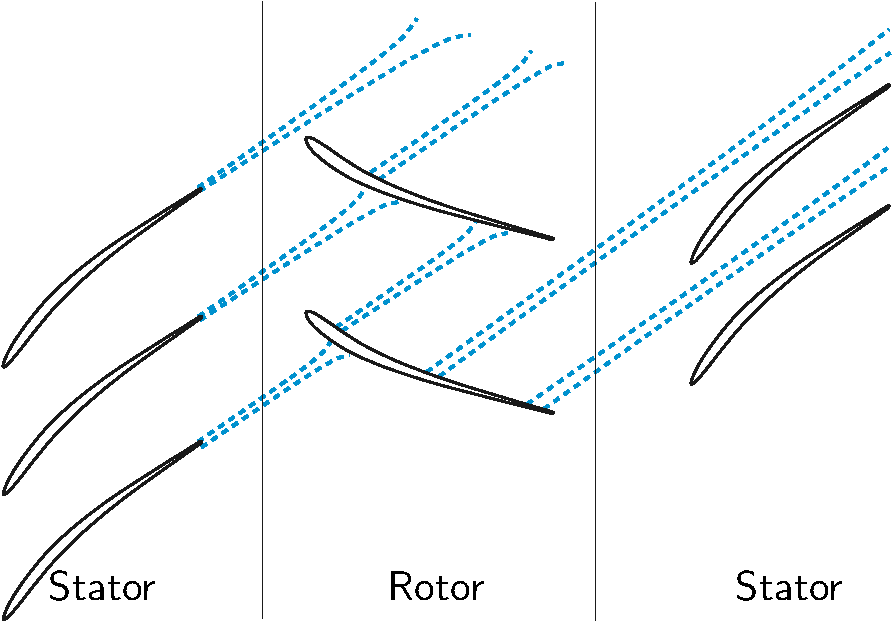
\includegraphics[width=.3\textwidth]{CLOCKING_EFFECT_1.pdf}}
    \subfigure{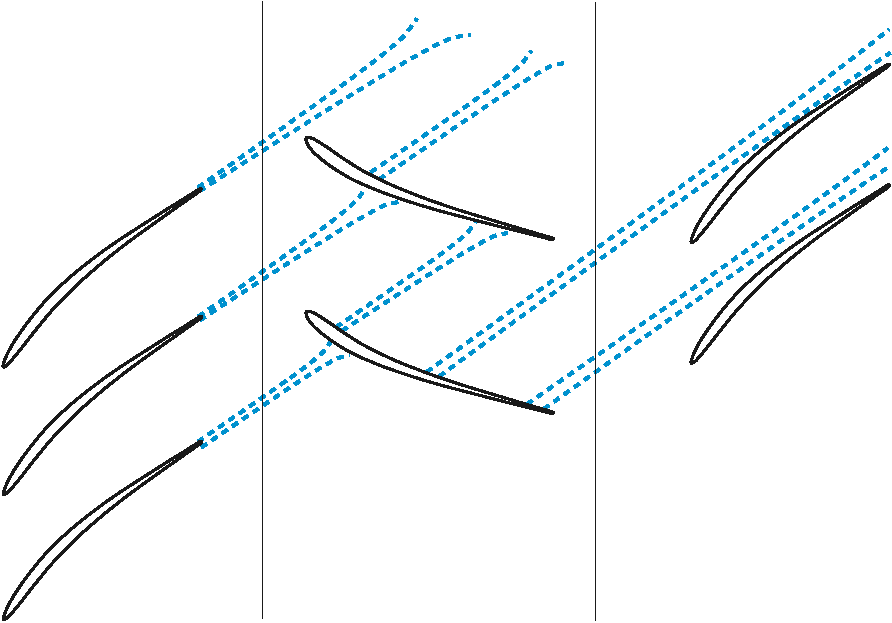
\includegraphics[width=.3\textwidth]{CLOCKING_EFFECT_2.pdf}}
    \subfigure{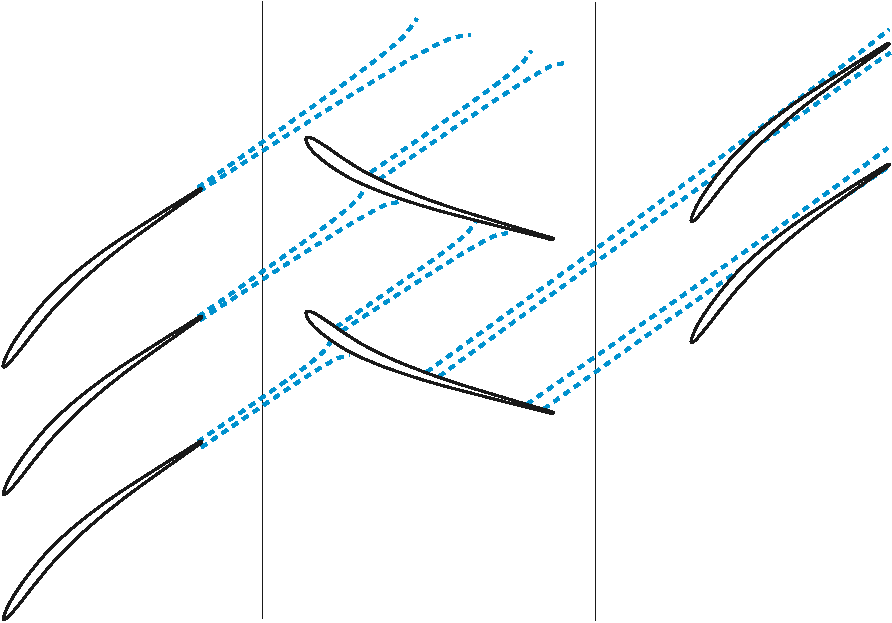
\includegraphics[width=.3\textwidth]{CLOCKING_EFFECT_3.pdf}}
  \caption{Different clocking positions for a stator/rotor/stator
  configuration.}
  \label{fig:sm_nlh_clocking_effect}
\end{figure}
Fig.~\ref{fig:sm_nlh_clocking_effect} displays three subfigures showing three
different clocking position in a stator/rotor/stator configuration.
As both stator are fixed, their relative position is of 
prior interest. The wake that is generated behind the first stator
is cut by the rotor blades but however almost convected up to 
the stator row. The stator being fixed, the wake generated
behind the first stator is seen stationary by the second stator.
Hence, the importance of their relative position. Here, the
first clocking position does not provide unsteadiness to the
last stator while the third clocking position gives the highest
level of unsteadiness for the stator. \todo{papier qui justifie
l'importance du calcul du clocking}

The brute force to compute the clocking effect on a
configuration is to consider all relative positions. This means
that the geometry of the stator should be rotated for each new 
clocking position. The innovative thinking proposed in 
\citet{He2002} is to consider the clocking effect as a steady wave.
In fact, as both stator are fixed, a steady perturbation
generated behind the first stator is still steady in the second stator.
In terms of frequencies, a steady perturbation is a perturbations 
whose frequency is zero. In \citet{He2002} and \cite{Vilmin2009}, 
a perturbation with a very small frequency (close to machine precision)
is computed. The clocking effect can then be evaluated by
post-processing the Fourier coefficient of the zero frequency mode.

Recently, the clocking effects \citet{Vilmin2013a}
\todo{à cmopléter}

\paragraph{Extension to the Navier-Stokes equations}

\paragraph{Applications}
The NonLinear Harmonic method 
has been succesfully implemented
in the NUMECA-Fine/Turbo solver by 
\citet{Vilmin2006, Vilmin2007, Vilmin2009, Vilmin2013a}.\todo{a améliorer + ajout frozen turbulence}

The presented NonLinear Harmonic method is particularly interesting
as it allows to compute the unsteadiness using a small amount 
of steady equations ($2N + 1$, with $N$ the number of harmonics chosen).
However, as all the development have to be made in the frequency domain,
one has to develop a new frequency based CFD solver. To face this issue,
\citet{Hall2002} proposed a new approach, the Harmonic Balance Technique

% subsection nonlinear_harmonic_method (end)

\subsection{The NonLinear Frequency Domain method} % (fold)
\label{sub:the_nonlinear_frequency_domain_method}

\paragraph{Mono-frequential formulation}

\paragraph{Multi-frequential formulation}

\paragraph{Extension to the Navier-Stokes equations}

\paragraph{Applications}

\paragraph{Timeline}

% subsection the_nonlinear_frequency_domain_method (end)


\section{The Harmonic Balance method} % (fold)
\label{sec:sm_harmonic_balance}

Originally proposed by \citet{Hall2002}, the Harmonic Balance Techniques
relies on a simple observation: to develop spectral methods, and in
particular the NonLinear Harmonic method, one has made use of the Fourier
transform to efficiently represent an unsteady signal with a Fourier series.
However, the method needs to be resolved in the frequency domain meaning
that all the numerical techniques should be adapted: the numerical schemes,
the turbulent model and so on. The smart idea 
proposed by \citet{Hall2002} is to
cast back the steady frequential equations to the time domain
by using an inverse Fourier transform.

Let us write Eq.~\ref{eq:sm_nonlinear_convection_conservative} 
in a more general form:
\begin{equation}
	\frac{\partial u}{\partial t} + R (u) = 0,
	\label{eq:sm_nonlinear_convection_residual}
\end{equation}
with
\begin{equation}
	R(u) = \frac{\partial}{\partial x} \left( 
	\frac{u^2}{2} \right).
\end{equation}

\subsection{Mono-frequential formulation}
A finite Fourier series truncated at order $N$ is defined as:
\begin{equation}
	u = \sum_{k=-N}^{N} 
	\widehat{u}_k e^{i k \omega t}.
	\label{eq:sm_hall_dft}
\end{equation}
Injecting Eq.~\ref{eq:sm_hall_dft} in 
Eq.~\ref{eq:sm_nonlinear_convection_residual}, and since
the complex exponentials form an orthogonal basis, 
this leads to:
\begin{equation}
	i k \omega \widehat{u}_k + \widehat{R}_k = 0, \: k \in [-N, N].
	\label{eq:sm_hall_frequential_eq}
\end{equation}
Obviously, the term $\widehat{R}_k$ is the hardest to develop
due to the nonlinearities. Here, the Harmonic Balance approach
is clever. 
Instead of developing this term in the frequency domain
using the Fourier coefficients $\widehat{u}_k$ of $u$,
one can assume that $R(u)$ can be decomposed using its own Fourier series
truncated at order $N$:
\begin{equation}
	R(u) = \sum_{k=-N}^{N} 
	\widehat{R}_k e^{i k \omega t}.
\end{equation}
This is an approximation as due to the nonlinearities, 
terms of order greater than $N$ appears, consequently, 
these are neglected in the present
formulation . However, the cross coupling terms corresponding
of the term $u^\prime u^\prime$ of the NonLinear Harmonic 
approach are not neglected here and
the terms of order greater
than $N$ are already neglected as $u$ is only evaluated using 
at most $N$ harmonics. This is thus coherent.

In the same way as one uses Fourier coefficients to
evaluate the temporal signal,
one can reconstruct the Fourier coefficients using
temporal evaluations taken at evenly spaced timelevels
sampling the period $T = 2 \pi / \omega$ using the forward
Fourier transform. Moreover, 
according to the Nyquist-Shannon~\cite{Shannon1949} sampling theorem, 
at least $2N+1$ timelevels are needed to capture $N$ frequencies,
leading to:
\begin{equation}
	\widehat{u}_k = \frac{1}{2N+1} 
	\sum_{n=0}^{2N} u_n^\star e^{-i k \omega t_n}.
\end{equation}
If $E$ denotes the matrix composed of the elements 
$E_{k,n} = e^{-i k \omega t_n} / 2N+1$, one can write $\widehat{u}_k$
and $\widehat{R}_k$ as:
\begin{equation}
	\begin{split}
		\widehat{u}_k &= E u^\star \\
		\widehat{R}_k &= E R^\star,
	\end{split}
\end{equation}
where $u^\star$ and $R^\star$ 
denote the vectors formed of all the evaluations of respectively $u$
and $R$,
made at the $2N+1$ timelevels. $E$ is thus the inverse Fourier operator.
Note that conversely, using the Fourier operator $E^{-1}$:
\begin{equation}
	\begin{split}
		u^\star &= E^{-1} \widehat{u}_k \\
		R^\star &= E^{-1} \widehat{R}_k.
	\end{split}
\end{equation}
Injecting the matrix formulation in Eq.~\ref{eq:sm_hall_frequential_eq}
gives:
\begin{equation}
	i K \omega E u^\star + E R^\star = 0,
\end{equation}
where $K$ is a diagonal matrix formed of all the $k \in [-N, N]$
Now multiplying the equation by the Fourier operator $E^{-1}$:
\begin{equation}
	i \omega E^{-1} K E u^\star + R^\star = 0,
\end{equation}
where $R^\star$ can now be substituted:
\begin{equation}
	\fbox{$
		i \omega E^{-1} K E u^\star + 
		\displaystyle \frac{\partial}{\partial x}
		\frac{(u^\star)^2}{2} = 0
	$}
\end{equation}
What happened here is that instead of developing $R(u)$
in the frequency domain, which is tedious, this term is kept
as it is through all the development process. 
Since $R(u)$ only includes spatial derivatives, no additional terms
rise from the Fourier decomposition. Hence, multiplying it
by the Fourier operator leads to the unity matrix. It is
simply evaluated at $2N+1$ timelevels.

The result is $2N+1$ steady equations coupled by a
source term that appears as a spectral
operator defined as:
\begin{equation}
	D_t = i \omega E^{-1} K E
\end{equation}

% subsection harmonic_balance_technique_of_hall (end)

% section state_of_the_art (end)

% chapter spectral_methods (end)
%!TEX root = ../main.tex
\section{choro} % (fold)
\label{sec:choro}

Without loss of generality one can
consider two rows (labeled $1$ and $2$) with a 
rotation rate equal to respectively $\Omega_1$ and $\Omega_2$ as
depicted in Fig.~\ref{fig:chorochronicity}.
$A$ and $B$ are two fixed observer in their respective reference
of frame. The cylindrical coordinate system is chosen.

\begin{figure}[htbp]
  \centering
  \includegraphics*[width=0.60\textwidth]{./CHOROCHRONICITY.pdf}
  \caption{Inter-blade dephasing}
  \label{fig:chorochronicity}
\end{figure}

The translation on the theta axis due to the different rotation rates can be 
written as:
\begin{equation}
    X_A (t + \delta t) = X_A (t) +  \Omega_1 \delta t \cdot \vec{e_\theta},
    \label{eq:choro_pos_A}
\end{equation}
and
\begin{equation}
    X_B (t + \delta t) = X_B (t) +  \Omega_2 \delta t \cdot \vec{e_\theta}.
    \label{eq:choro_pos_B}
\end{equation}

By subtracting Eq.~\eqref{eq:choro_pos_B} and Eq.~\eqref{eq:choro_pos_A}
one gets:
\begin{equation}
    X_A (t + \delta t) - X_A (t) = X_B (t + \delta t) - X_B (t) + (\Omega_2 - \Omega_1) \delta t \cdot \vec{e_\theta}.
\end{equation}



% section choro (end)
% 
% # Validation
%     * Presentation of the toy problems
%        - Convection equation
%        - Rotating block configuration
%     * Advantages
%         - capturing a sinusoidal flow
%         - capturing a wake / clocking effects
%     * Drawbacks
%         - non evenly spaced timelevels
%         - signal to capture (wake / sinus / step function)
%!TEX root = ../main.tex
\chapter{Validation} % (fold)
\label{cha:validation}

\section{Presentation of the toy problems}

To demonstrate the capacities and the limitations of
the harmonic balance approach, two toy problems are set up.
The first one solves the constant convection equation within 
a harmonic balance framework, the second one is a laminar
Navier-Stokes rotating blocks configuration.

\subsection{Convection equation problem} % (fold)
\label{sub:convection_equation_problem}

The harmonic balance source term is an alternative to
a classical time marching scheme for periodic phenomenon.
The simplest unsteady equation
that can be formulated is the constant convection equation:
\begin{equation}
  \label{eq:convection}
  \frac{\partial u}{\partial t} + c \frac{\partial u}{\partial x} = 0,
\end{equation}
where $c$ denotes the constant velocity and $u$ the transported quantity.
If we impose an unsteady periodic inlet,
we obtain a simple test case for harmonic balance approach. Any kind
of input can be simulated allowing to fully investigate the properties of 
the method.

Moreover, this equation is interesting as the analytical solution is simple
and known for any input. In fact, the solution only depends on the 
initial and/or boundary conditions:
\begin{equation}
  \label{eq:solconvanalytic}
    u(x, t) = u_0(x - ct)
\end{equation}
where $u_0$ is the boundary condition. Moreover, as the equation
is simple enough, it will be easy to discriminate the effects of the
harmonic balance source term.

The convection equation is solved in a 1D cartesian mesh.
A $4$\textsuperscript{th} order centered finite
difference scheme is used to evaluate the spatial derivative:
\begin{equation}
    \left. \frac{\partial u}{\partial x} \right)_{t=q}^{x=i} \approx 
    \frac{-u^{i+2}_{q} + 8 u^{i+1}_{q} - 8 u^{i-1}_{q} + u^{i-2}_{q}}{12\Delta x},
    \label{eq:convection_center4}
\end{equation}
where $u_i^q$ is the sum of the velocity for  
all harmonic balance instants as defined in Eq.~\eqref{eq:hb_concatenation},
evaluated at position $i$ within pseudo-iteration $q$.
A $4$ step Runge-Kutta method is then use to time 
march the equation to the steady state with the coefficients $\alpha_0 = 0$,
$\alpha_1 = 1/4$, $\alpha_2 = 1/3$, $\alpha_3 = 1/2$ and $\alpha_4 = 1$.
The k\textsuperscript{th} step is evaluated by:
\begin{equation}
    u_k = u_q - \alpha_k \Delta t \left [ 
          c \left. \frac{\partial u_{k-1}}{\partial x} \right)_{t=t_q + \alpha_{k-1} \Delta t}
          + D_t(u_q)
          \right],
    \label{eq:convection_rk4}
\end{equation}
where the HB source term $D_t(u_q)$ is computed using Eq.~\eqref{eq:dt}. 

As we use 
an explicit time marching scheme, the CFL number is set to $1$ to ensure stability.
The mesh is composed of $2000$ grid points, which proved to be converged.
The period of injection is chosen so that, when the temporal frequency is
set to $1$, only one pattern 
appears at a time in the mesh
as shown in Fig.~\ref{fig:convection_injection_paper} for a Gaussian function.
This is done by setting the biggest temporal period $T$ to:
\begin{equation}
   T = \frac{L_x}{c},
\end{equation}
where $L_x$ is the size of the mesh.


As the harmonic balance computations are steady computations linked 
by a source term, 
different boundary conditions, as done in~\cite{Dufour2010},
have to be set to impose a periodic injection. Two ghost cells
are used to maintain the spatial $4$\textsuperscript{th} order scheme 
at the left
boundary condition.
\begin{figure}[htbp]
  \begin{center}
    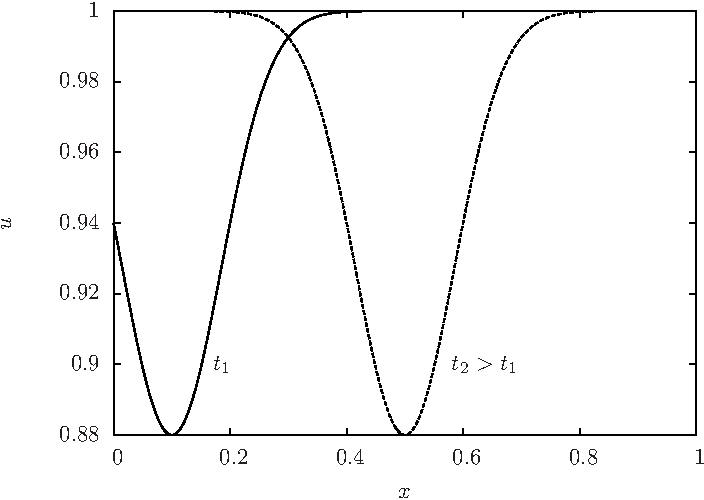
\includegraphics[width=.5\textwidth]{GAUSSIAN_INJECTION_PAPER.pdf}
  \end{center}
  \caption{Convection of the Gaussian function in the 1D cartesian mesh.}
  \label{fig:convection_injection_paper}
\end{figure}
For the right boundary condition, imposing a periodicity condition is
numerically stiff. For this reason, the scheme is degenerated 
to an upwind scheme to avoid wave reflections. The upwind scheme is degenerated to
a 2\textsuperscript{nd} order, one cell before and at first order on the 
last cell:
\begin{align}
    \left. \frac{\partial u}{\partial x} \right)_{t=q}^{x=m-1} &\approx 
    \frac{3 u^{m-1}_{q} - 4 u^{m-2}_{q} + u^{m-3}_{q}}{2\Delta x}, \\
    \left. \frac{\partial u}{\partial x} \right)_{t=q}^{x=m} &\approx 
    \frac{u^{m}_{q} - u^{m-1}_{q}}{\Delta x},
\label{eq:upwind_scheme}
\end{align}
where $m$ is the total number of grid points. This is much better than a periodicity
condition as the convected function suffers from diffusion and dispersion (even if the
mesh is small enough) that is not compatible with the injected function.

% chapter validation (end)
% 
% # Improving the method
%     * algorithm to automatically choose the timelevels
%!TEX root = ../main.tex

%     * convergence of spectral methods : analyzing the spectrum of the wake
%     * partial conclusion: we may go to industrial applications
% 
% # application to the aeroelasticity of contra-rotating open rotors
%     * validation of the proposed approach (STCF 11)
%!TEX root = ../main.tex
\chapter{Application to the aeroelasticity of contra-rotation open rotors} % (fold)
\label{cha:application_to_the_aeroelasticity_of_contra_rotation_open_rotors}

\lhead{Chapitre ??. \emph{Application to the aeroelasticity of CRORs}}

\section{Validation of the proposed approach} % (fold)
\label{sec:validation_of_the_proposed_approach}


For external-flow aeroelasticity, the HB approach has 
been thoroughly validated~\cite{Gopinath2005,Sicot2008,Woodgate2009,Dufour2010}, 
mostly for the AGARD test cases of Davis~\cite{Davis1982}. 
However, experimental data for turbomachinery aeroelasticity are more scarce: 
the Standard Aeroelastic Configurations experiments 
of Fransson~\textit{et al.}~\cite{Fransson:1999uq} are the 
reference in this respect, and have been widely used 
to validate different numerical approaches~\cite{Sbardella:2001fk,
Duta:2002uq,Campobasso:2003fk,Cinnella2004,mcbean2005}. 


The $11$\textsuperscript{th} standard configuration is a
turbine stator composed of 20~blades, and tested at EPF-Lausanne
in the late 1990's by Fransson~\emph{et al.}~\cite{Fransson:1999uq}.
The test cascade is placed in a 
annular test rig as depicted in~Fig.\ref{fig:annular_channel}
\begin{figure}[htbp]
  \centering
  \includegraphics*[width=0.40\textwidth]{./ANNULAR_CHANNEL.pdf}
  \caption{Annular test rig for the standard configurations}
  \label{fig:annular_channel}
\end{figure}
The experimental results have been found to be highly reproducible and
therefore suitable for code validation~\cite{Fransson:1999uq}.  


% geometry presentation
The geometry profile and the results are available over the
internet~\cite{stcf11web}.  To allow local validation of the steady
flow, the isentropic Mach number is given at blade wall.

The blades oscillate harmonically in the first bending mode
at a reduced frequency of $f_{c} =\pi \cdot c \cdot
f/U_{outlet, exp} = 0.2134$ for the subsonic case and $0.1549$ for the
transonic case. Aeroelastic
results are available such as the first harmonic of the unsteady pressure
coefficient at blade walls (amplitude and phase), for several nodal
diameters. The integrated
results, such as the damping, strongly vary under small changes in the
local distribution. It is therefore recommended to look at the local
distributions.
 
% mesh presentation
The blade passage is meshed using an O4H topology (Fig.~\ref{fig:stcf11_mesh}).  
The number of grid points along the blade
chord axis is~160 and the computed $y^+$ at the walls is $\mathcal{O}(1)$. % proving
The blade has the same profile along the spanwise direction and no
twist. Therefore, a 2.5D mesh is used with five points in the radial direction, with a spanwise
extent representing $1\%$ of the chord. 

% boundary conditions
The boundary conditions used for this case are: (i)~an
injection condition  for the inlet (with a relative flow angle
set to the  experimental value), (ii)~a constant static pressure
condition for the outlet,  (iii)~an adiabatic no-slip condition on
blade walls, and (iv)~periodic or phase-lagged conditions for azimuthal boundaries depending on the  
prescribed IBPA.

% numerical parameters
Turbulence is modeled using the one-equation model of
Spalart-Allmaras~\cite{Spalart1992}.  The third-order upwind Roe
scheme~\cite{Roe1981} is used to compute the convective fluxes.
The maximum
CFL number is set to~20 for the steady computations,  the inner loop
of the DTS scheme and the HB simulations.  For the DTS scheme,  
convergence in time discretization is obtained
after 20~periods using 128~instants per period.  Iterative convergence 
for the inner loop is considered achieved when the normalized
residuals drop by $5\cdot 10^{-2}$ (within a maximum of
50~sub-iterations).

\subsection{Subsonic Case}
The measured inlet Mach number is $0.31$ and the isentropic outlet Mach number is $0.69$.
% steady results
Steady results for the isentropic Mach number at blade walls are compared to the experimental data in 
Fig.~\ref{fig:stcf11_rans_subsonic}.  For this flow regime, the flow
remains subsonic.
On the pressure side, the flow accelerates all the way
to the trailing edge of the blade. On the suction side, the flow
accelerates until a maximum speed at $\approx 40~\%$ of the chord and
then decelerates (Fig.~\ref{fig:stcf11_subsonic_field_mis_bw}).
The agreement with the experimental data is fair. However, an
over-prediction of the isentropic Mach number is observed on the suction
side.  This discrepancy is also reported in the literature (see
Ref.~\cite{Fransson:1999uq} for instance).
\begin{figure}[htb]
  \centering
  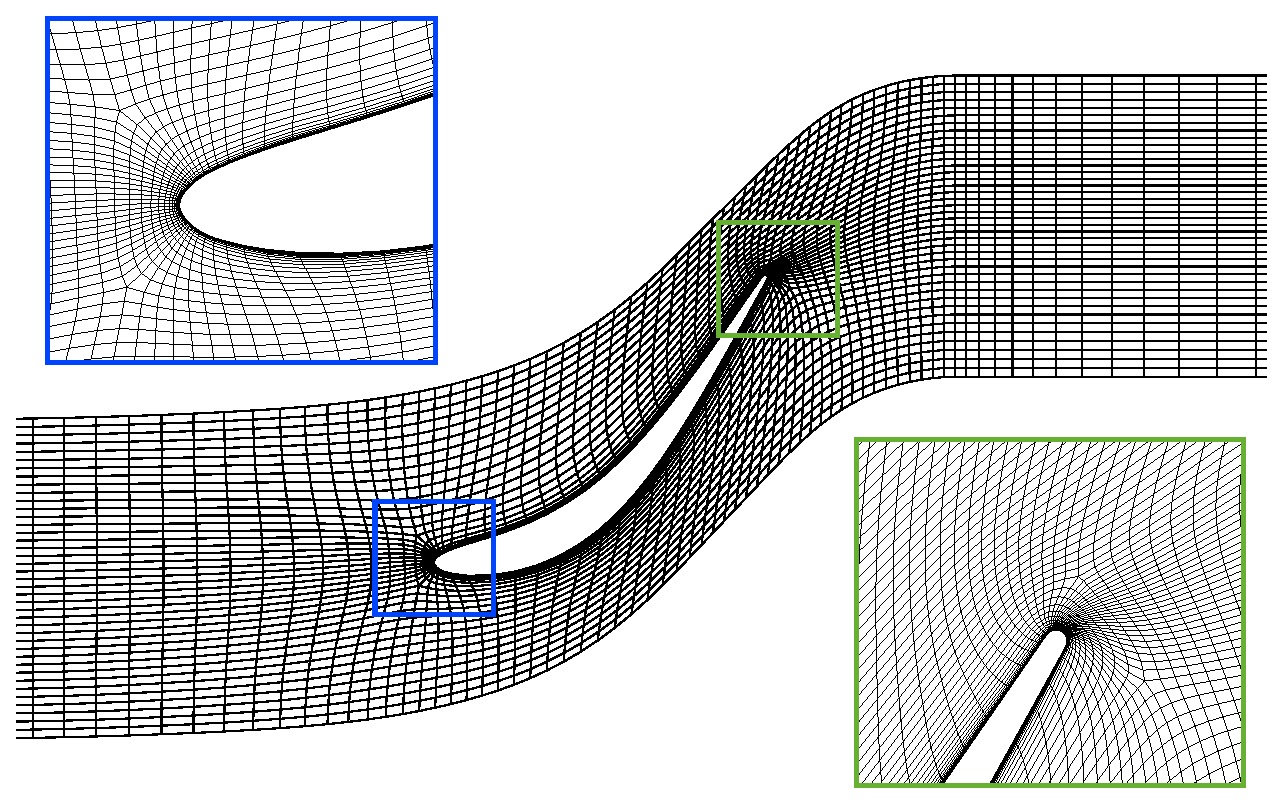
\includegraphics[width=.46\linewidth]{STCF11_MESH.eps}
  \caption{STCF 11 mesh}
  \label{fig:stcf11_mesh}
\end{figure}

\begin{figure}[htb]
  \centering
  \begin{minipage}[b]{.46\linewidth}
    \centering
    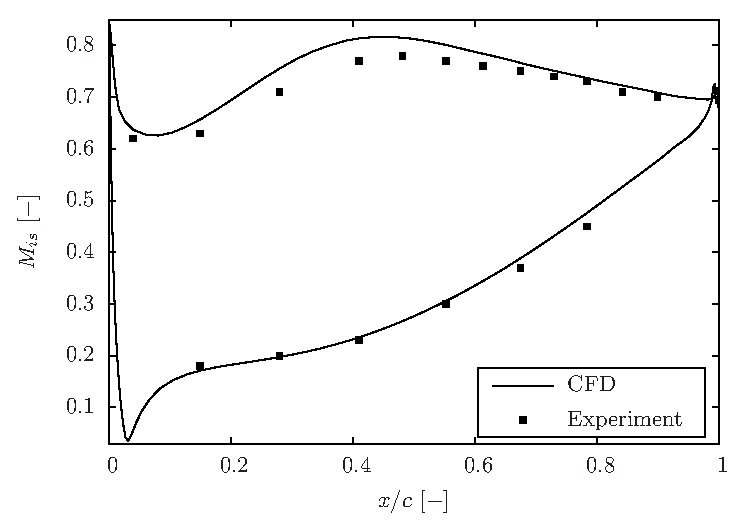
\includegraphics[width=\textwidth]{STCF11_RANS_SUBSONIC.eps}
    \caption{Steady results of the isentropic Mach number at blade
      walls, subsonic case}
    \label{fig:stcf11_rans_subsonic}
  \end{minipage}\quad
  \begin{minipage}[b]{.46\linewidth}
    \centering
    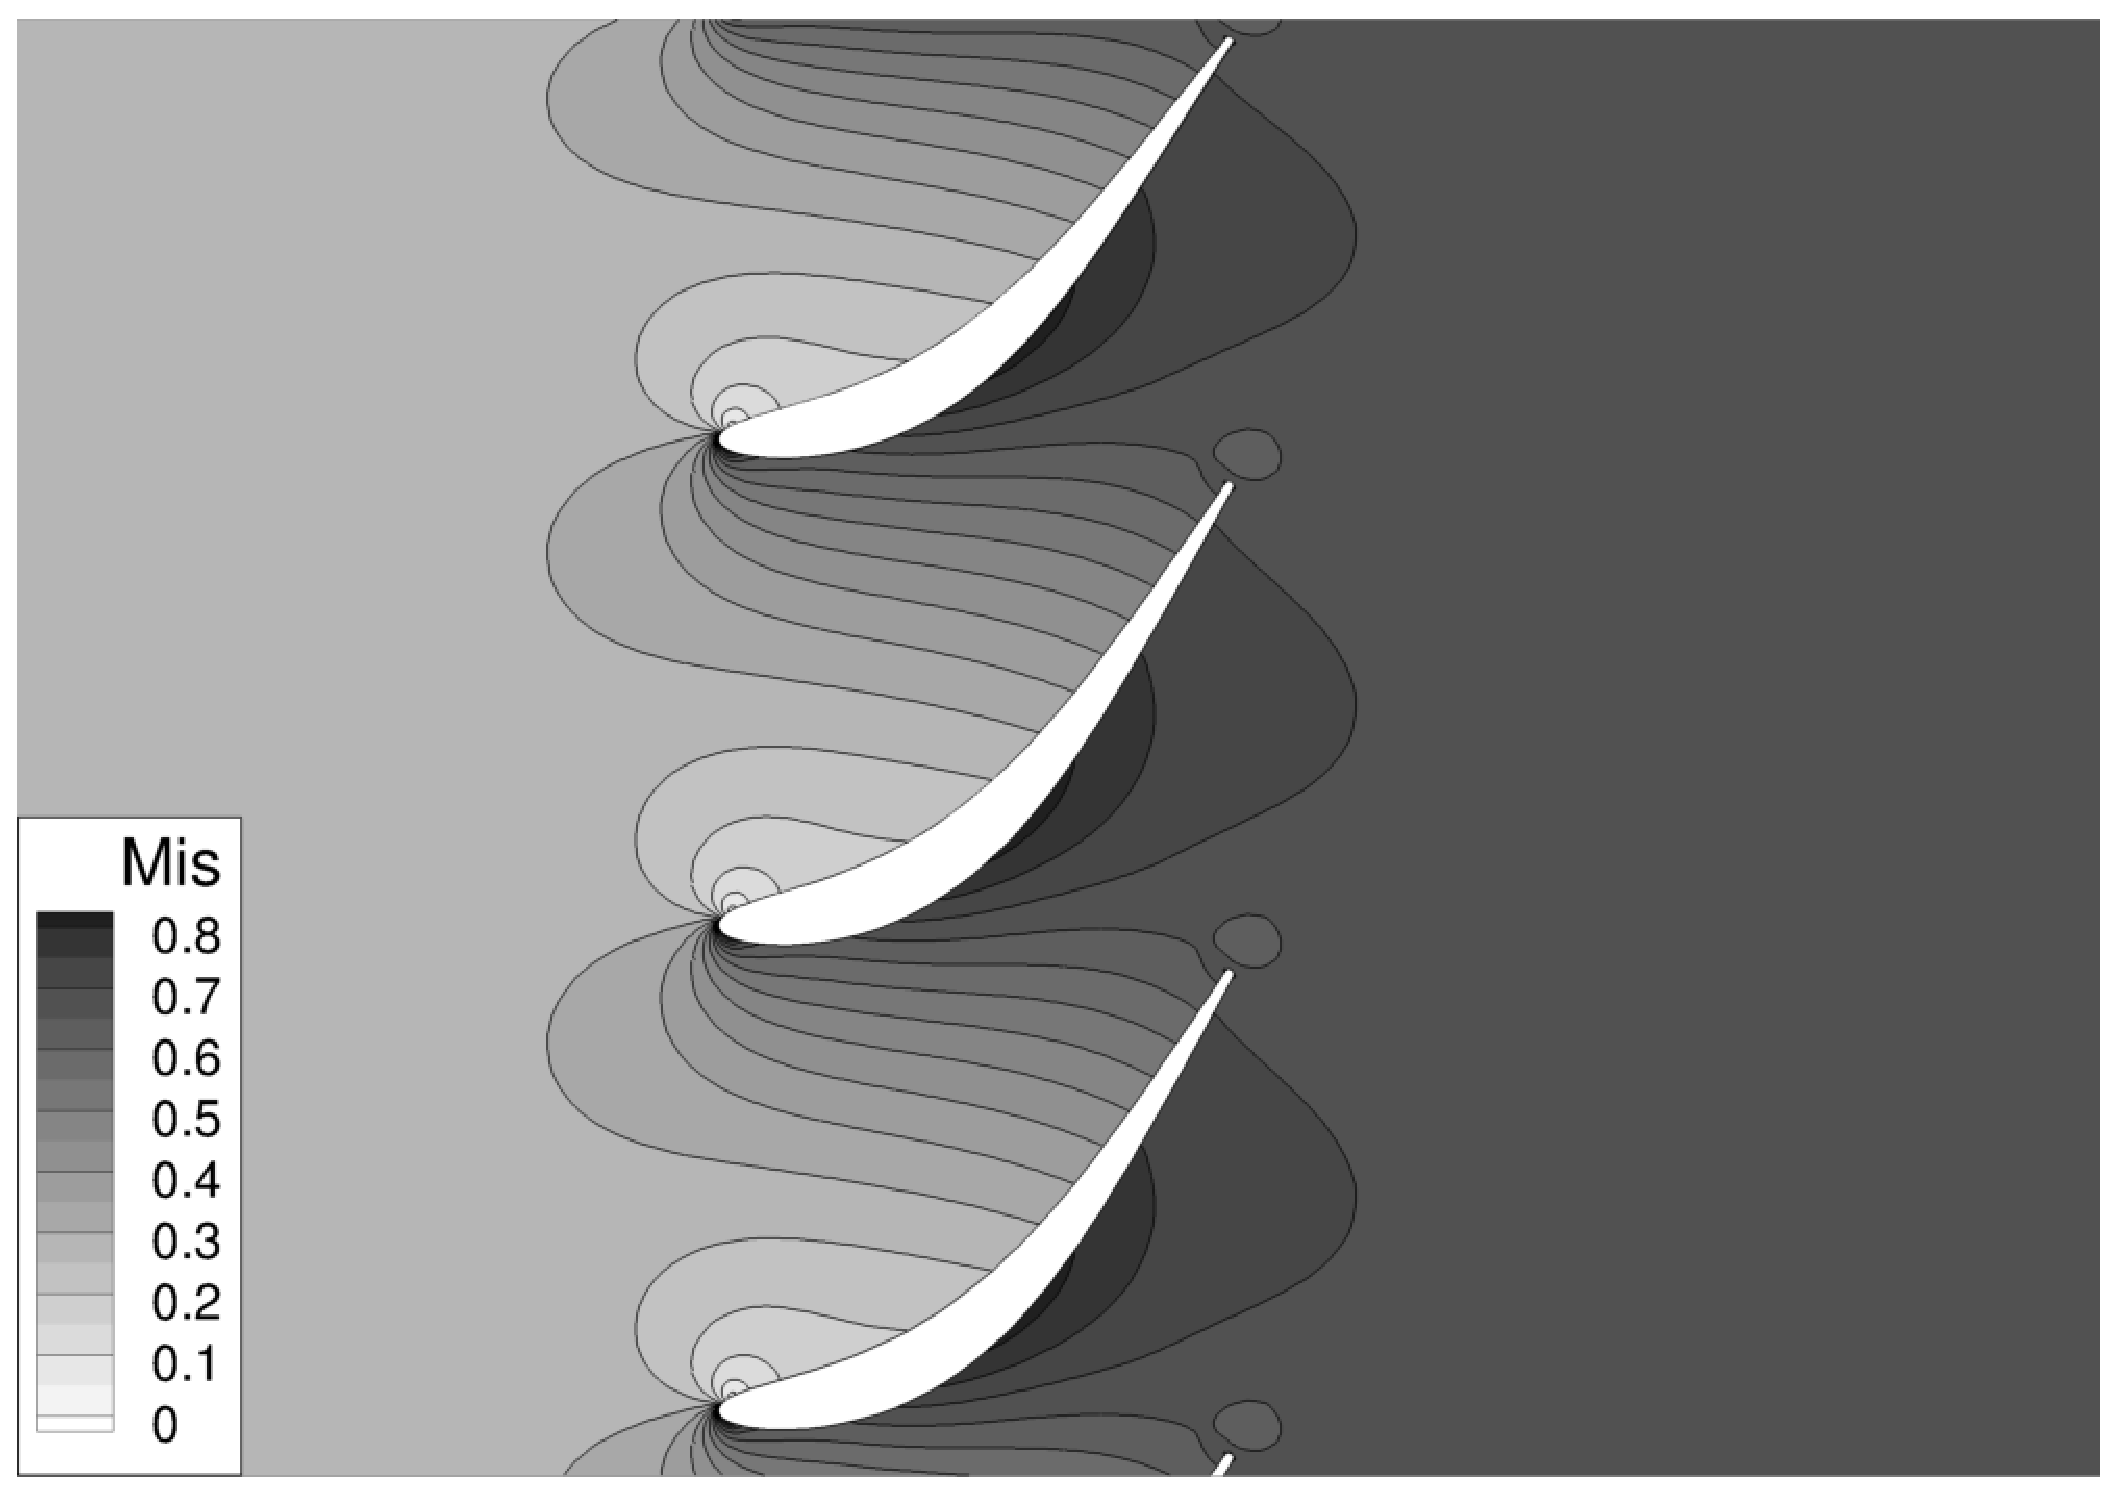
\includegraphics[width=\textwidth]{STCF11_SUBSONIC_FIELD_MIS_BW.eps}
    \caption{Steady isentropic Mach number contours, subsonic case}
    \label{fig:stcf11_subsonic_field_mis_bw}
  \end{minipage}
\end{figure}

% unsteady results
The aeroelastic experimental data are compared to the present results
obtained with both the DTS and the HB approach. To explore the range
of nodal diameters with the HB method, an incremental approach is used
where each nodal diameter simulation is used to initialize the next
one.  Considering the opposite phase vibration case (the 10\textsuperscript{th} nodal diameter), 
the amplitude and the phase of the pressure coefficient are
presented in Fig.~\ref{fig:stcf11_ael_subsonic_ibpa_180_paper}.
With only one harmonic (\emph{i.e.},~three instants), the HB results
are superimposed on the DTS ones. Moreover, the numerical results are
in fair agreement with the experimental data for the
amplitude. However, for the phase, the sign change on the
suction side is predicted at about $60~\%$ of the chord, whereas the
experimental location is about 25~\%.
\begin{figure}[htb]
  \centering 
  \begin{tabular}{cc}
    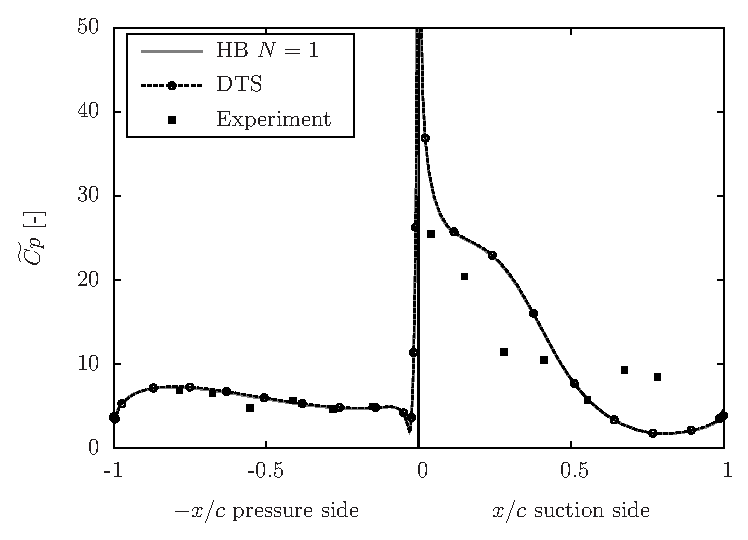
\includegraphics[width=.45\textwidth]{STCF11_AEL_SUBSONIC_IBPA_180_Cp_paper.eps}
    &
    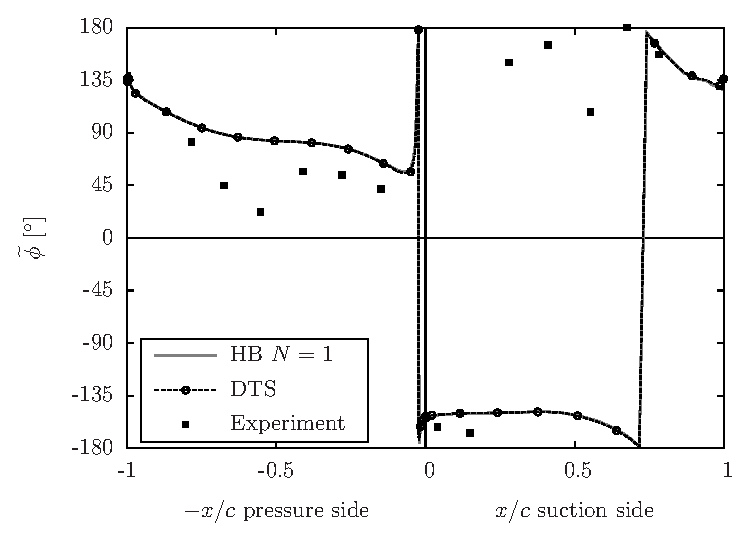
\includegraphics[width=.45\textwidth]{STCF11_AEL_SUBSONIC_IBPA_180_Phi_paper.eps}\\
    (a) Amplitude part & (b) Phase part
  \end{tabular}
  \caption{Wall pressure harmonic analysis for an opposite phase vibration, subsonic case}
  \label{fig:stcf11_ael_subsonic_ibpa_180_paper}
\end{figure}


The results for the  nodal  diameter $-2$ are shown
in Fig.~\ref{fig:stcf11_ael_subsonic_ibpa_324_paper}. The HB and DTS data
are superimposed, and are in fair agreement with the experiments. The
amplitude levels are well captured and the phase prediction is
slightly improved over the opposite phase case.
\begin{figure}[htb]
  \centering 
  \begin{tabular}{cc}
    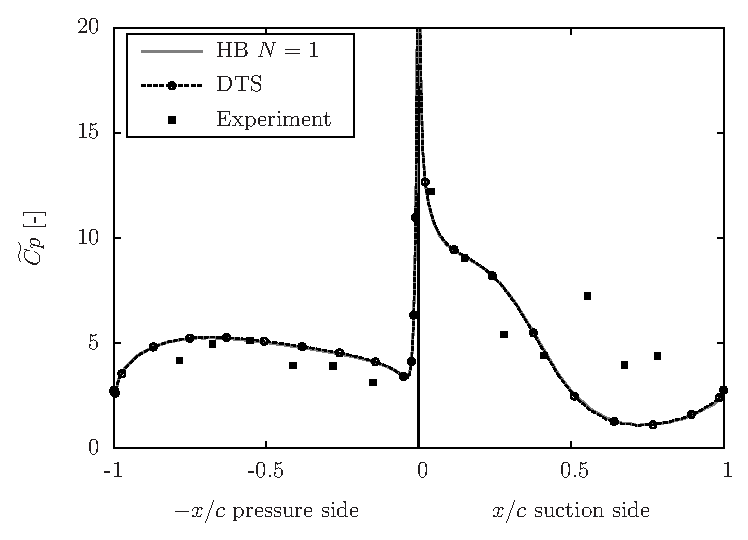
\includegraphics[width=.45\textwidth]{STCF11_AEL_SUBSONIC_IBPA_324_Cp_paper.eps}
    &
    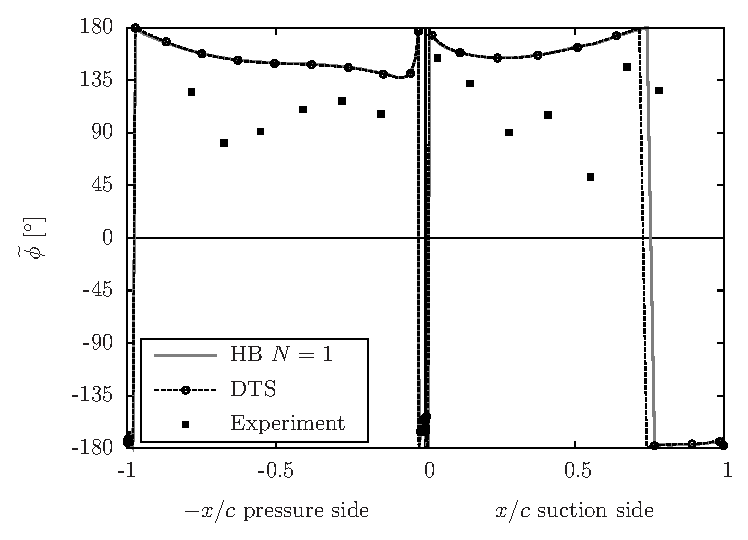
\includegraphics[width=.45\textwidth]{STCF11_AEL_SUBSONIC_IBPA_324_Phi_paper.eps}\\
    (a) Amplitude part & Phase part
  \end{tabular}
  \caption{Wall pressure harmonic analysis for \mbox{$n_d=-2$}, subsonic case}
  \label{fig:stcf11_ael_subsonic_ibpa_324_paper}
\end{figure}

The damping obtained from the previous calculations is depicted 
in Fig.~\ref{fig:stcf11_subsonic_damping}.  Also plotted are the results
from Fransson~\emph{et al.}~\cite{Fransson:1999uq}, obtained with both
potential, linear Euler, non-linear Euler and non-linear viscous codes.
The results for all IBPAs are given for the potential code but only $\beta=180^\circ$ is provided for the other codes~\cite{Fransson:1999uq}.
These are the only damping results for the
subsonic case known by the authors.  Since the local variations are
superimposed for the DTS and the HB approaches, so are the damping.
The present
results show similar trends and levels to those of Fransson~\emph{et al.} 
\begin{figure}[htb]
  \centering
  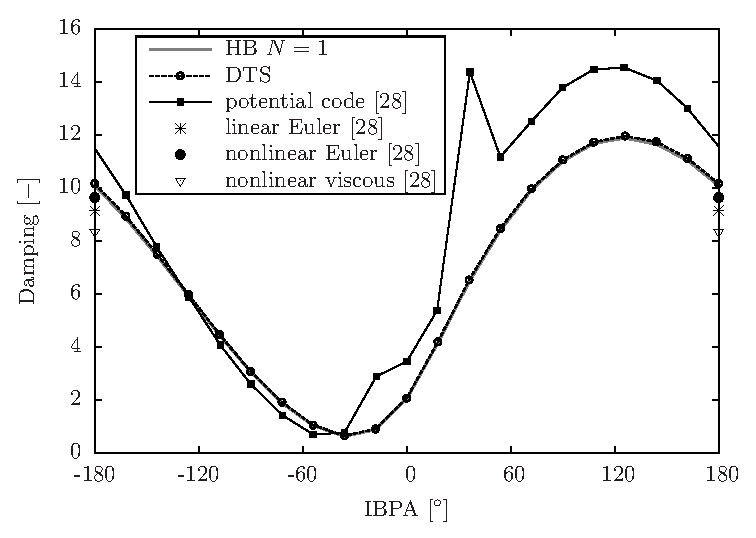
\includegraphics[width=.46\linewidth]{STCF11_SUBSONIC_DAMPING.eps}
  \caption{Aerodynamic damping coefficient versus IBPA, subsonic case}
  \label{fig:stcf11_subsonic_damping}
\end{figure}



\subsection{Transonic Condition}
The outlet isentropic Mach number is $0.99$ for an inlet Mach number of $0.4$. 
This case, for which experimental uncertainties are available, 
has been largely addressed in the literature 
(see for instance Refs.~\cite{Sbardella:2001fk,Duta:2002uq,Campobasso:2003fk,Cinnella2004}). 
This test case is challenging in terms of nonlinearities as a separation bubble and a shock are present.

Steady results of the isentropic Mach number are shown in
Fig.~\ref{fig:stcf11_rans_transonic}.  For this flow regime,
a small separation
bubble develops on the suction side at the leading edge~(cf.~Fig.~\ref{fig:stcf11_transonic_field_mis_bw}).  The flow then accelerates, followed by a passage shock.  
The experimental data suggests that the shock appears
sooner on the suction side than in the computations; all the results 
reported in the literature exhibit similar discrepancies (see
Refs.~\cite{Fransson:1999uq,Sbardella:2001fk,Duta:2002uq,Campobasso:2003fk,Cinnella2004}). 
Otherwise, the present results are in fair agreement with experimental data.
\begin{figure}[htb]
  \centering
  \begin{minipage}[b]{.46\linewidth}
    \centering
    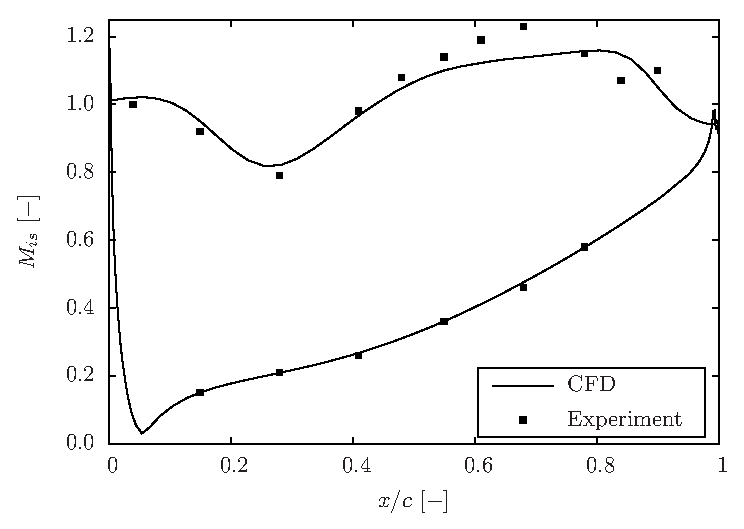
\includegraphics[width=\textwidth]{STCF11_RANS_TRANSONIC.eps}
    \caption{Steady results of the isentropic Mach number at blade
      wall, transonic case}
    \label{fig:stcf11_rans_transonic}
  \end{minipage}\quad
  \begin{minipage}[b]{.46\linewidth}
    \centering
    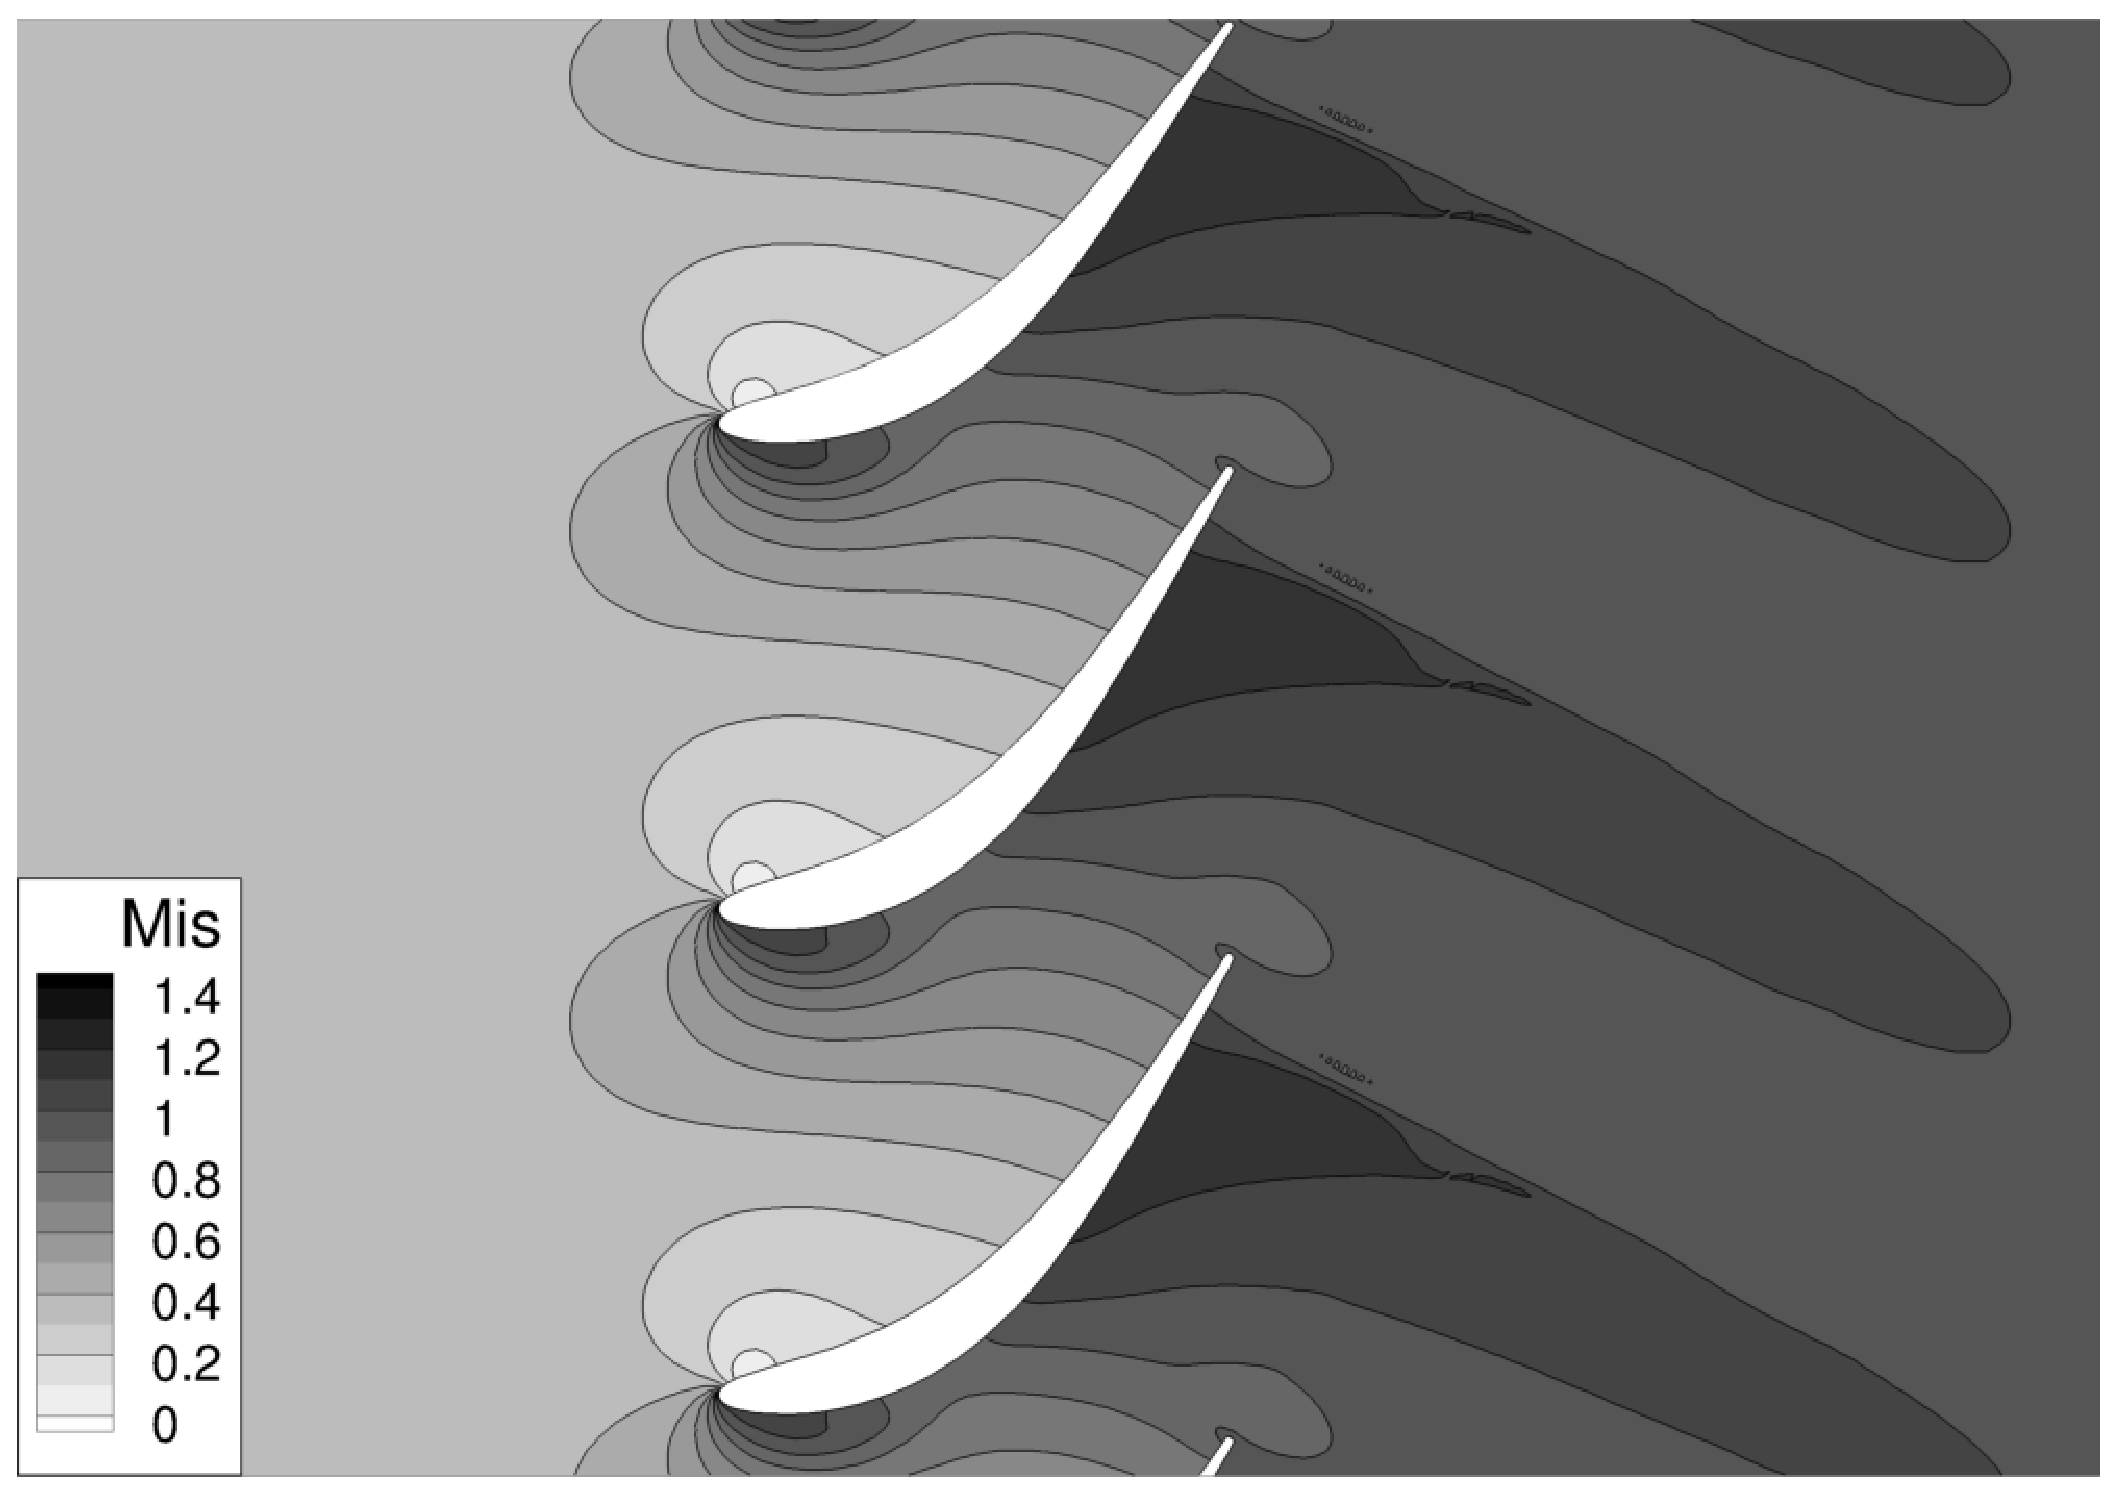
\includegraphics[width=\textwidth]{STCF11_TRANSONIC_FIELD_MIS_BW.eps}
    \caption{Steady isentropic Mach number contours, transonic case}
    \label{fig:stcf11_transonic_field_mis_bw}
  \end{minipage}
\end{figure}

% unsteady results
The aeroelastic experimental data are compared to the present results
obtained with both the DTS and the HB approach.  Considering the opposite phase vibration case (the 10\textsuperscript{th} nodal diameter), 
the amplitude and the
phase of the pressure coefficient are presented in
Fig.~\ref{fig:stcf11_ael_transonic_ibpa_180_paper}. Also plotted are the results of
Cinnella~\emph{et~al.}~\cite{Cinnella2004}, computed with a nonlinear viscous
approach using the Spalart-Allmaras turbulence model. The present HB and the DTS
results are superimposed, which indicates that the one harmonic HB solution is able
to reproduce the unsteady nonlinear effects without increasing the
number of harmonics. This observation is only valid near the wall,
before the harmonics are created naturally by the flow, due to the
nonlinear effects. The results are in good agreement with
the experimental data and display the same trends as that of
Cinnella~\emph{et~al.}  A slight discrepancy can be observed within the shock
region, where the amplitude and the phase phenomena are predicted
further than the experiments indicate.  This can be attributed to the poor
prediction of the shock position and hence the poor prediction
of its interaction with the motion of the blade.
\begin{figure}[htb]
  \centering
  \begin{tabular}{cc}
    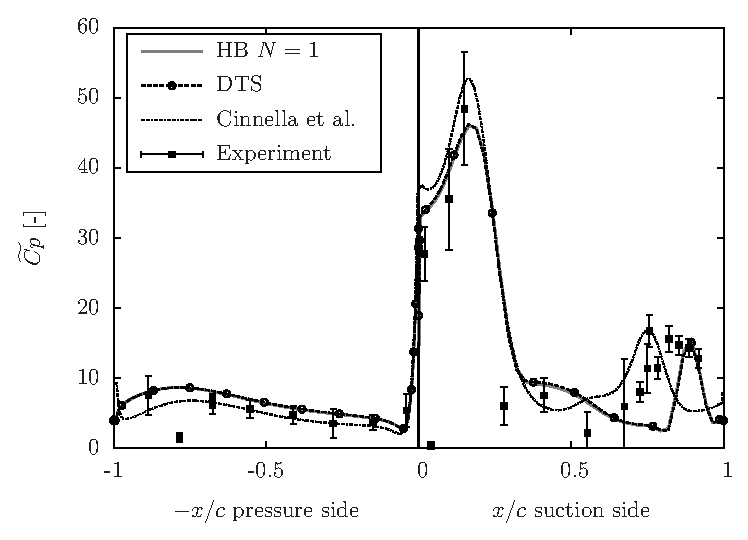
\includegraphics[width=.45\textwidth]{STCF11_AEL_TRANSONIC_IBPA_180_Cp_paper.eps}
    &
    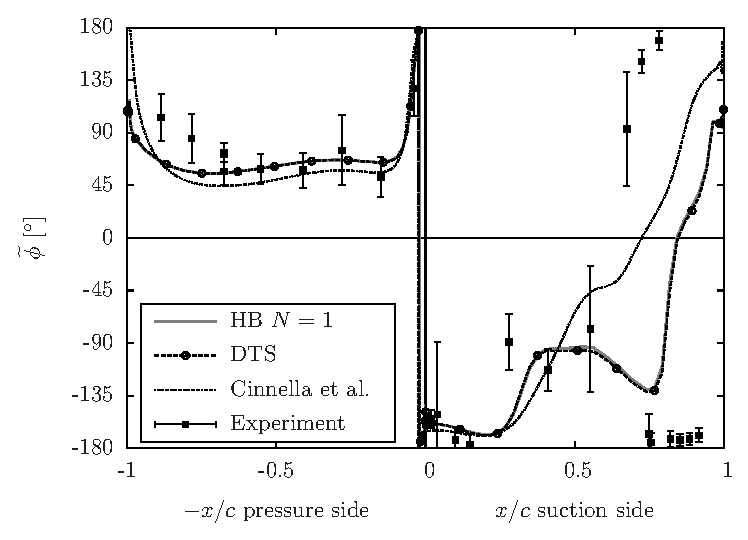
\includegraphics[width=.45\textwidth]{STCF11_AEL_TRANSONIC_IBPA_180_Phi_paper.eps}\\
    (a) Amplitude part & Phase part
  \end{tabular}
  \caption{Wall pressure harmonic analysis for an opposite phase vibration, transonic case}
  \label{fig:stcf11_ael_transonic_ibpa_180_paper}
\end{figure}

The results for the $-2$\textsuperscript{th} nodal diameter are also shown in
Fig.~\ref{fig:stcf11_ael_transonic_ibpa_324_paper}. Again,
the HB results are superimposed on the DTS ones. Moreover, these are in
good agreement with the experiments, considering the uncertainties of
the experimental data.
\begin{figure}[htb]
  \centering 
  \begin{tabular}{cc}
    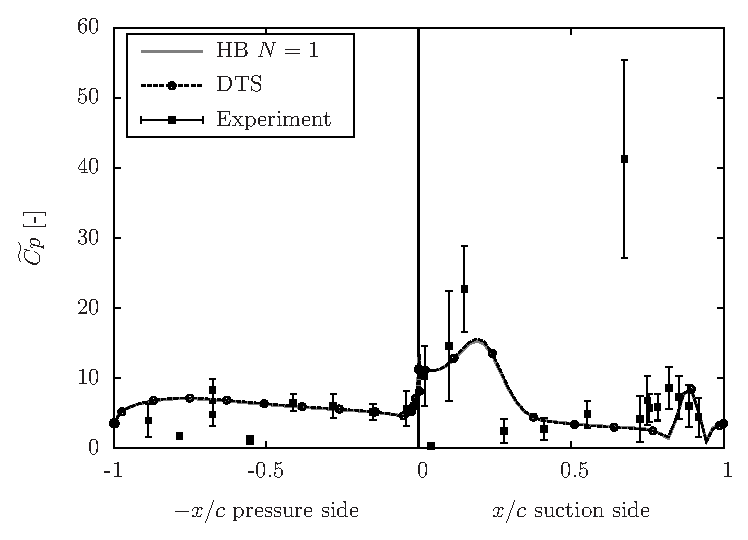
\includegraphics[width=.45\textwidth]{STCF11_AEL_TRANSONIC_IBPA_324_Cp_paper.eps}
    &
    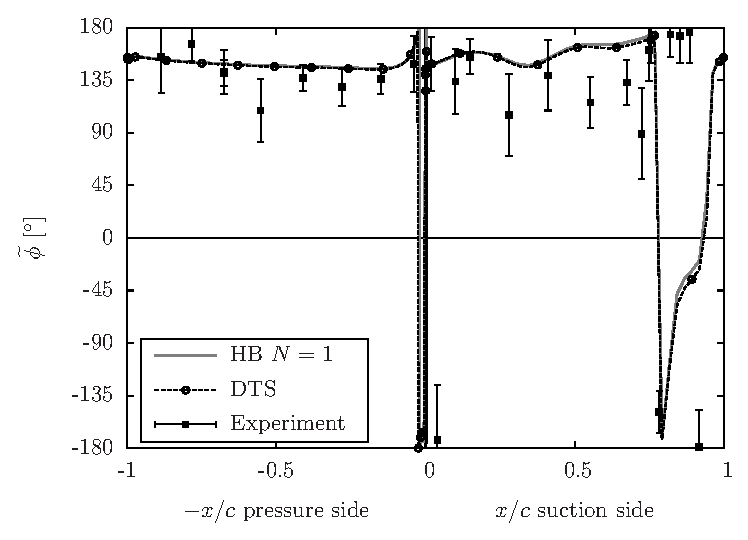
\includegraphics[width=.45\textwidth]{STCF11_AEL_TRANSONIC_IBPA_324_Phi_paper.eps}\\
    (a) Amplitude part & (b) Phase part
  \end{tabular}
  \caption{Wall pressure harmonic analysis for \mbox{$n_d=-2$}, transonic case}
  \label{fig:stcf11_ael_transonic_ibpa_324_paper}
\end{figure}

The damping is shown in Fig.~\ref{fig:stcf11_transonic_damping} for
the transonic case. Also plotted are the results from
Fransson~\emph{et al.} (potential code), and 
from Cinnella~\emph{et al.} (RANS). The scattering is much more severe
than for the subsonic case. The trends obtained with the RANS approaches are similar. However, the
discrepancies between the two RANS codes are significant in terms of
levels.
Recently, Vogt and Fransson~\cite{Vogt:2011fk} reported similar discrepancies 
for damping predictions of subsonic and transonic cascades, 
showing that the damping can be significantly affected by 
small local changes in the amplitude and/or the phase.
\begin{figure}[htb]
  \centering
  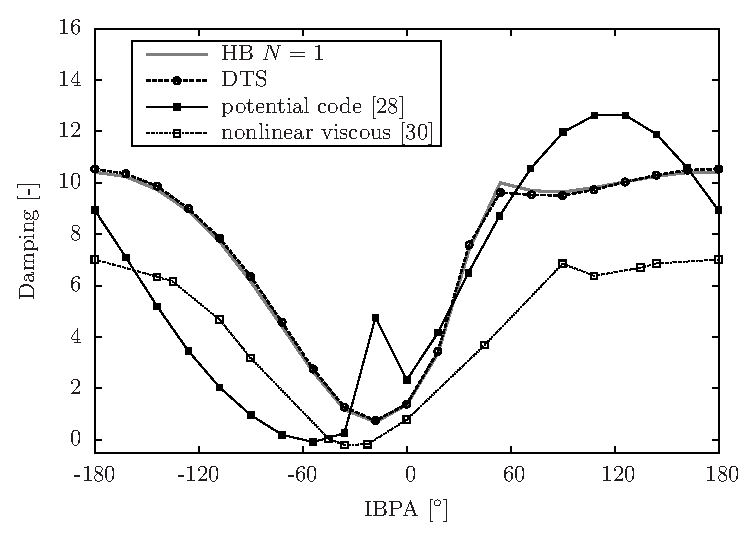
\includegraphics[width=.46\linewidth]{STCF11_TRANSONIC_DAMPING.eps}
  \caption{Aerodynamic damping coefficient versus IBPA, transonic
    case}
  \label{fig:stcf11_transonic_damping}
\end{figure}
In terms of computational efficiency, the HB method is 7 times faster
than the DTS  for all the IBPAs.

% section validation_of_the_proposed_approach (end)

% chapter application_to_the_aeroelasticity_of_contra_rotation_open_rotors (end)

%     * aeroelasticity of an isolated contra-rotating open rotor
%     * aeroelasticity of an installed contra-rotating open rotor


%----------------------------------------------------------------------------------------
%	THESIS CONTENT - APPENDICES
%----------------------------------------------------------------------------------------

\addtocontents{toc}{\vspace{2em}} % Add a gap in the Contents, for aesthetics

\appendix % Cue to tell LaTeX that the following 'chapters' are Appendices

% Include the appendices of the thesis as separate files from the Appendices folder
% Uncomment the lines as you write the Appendices

%!TEX root = ../main.tex
\chapter{Validation of the convection code}
\label{Appendix_convection_code}

%\input{./Appendices/AppendixB}
%\input{./Appendices/AppendixC}

\addtocontents{toc}{\vspace{2em}} % Add a gap in the Contents, for aesthetics

\backmatter

%----------------------------------------------------------------------------------------
%	BIBLIOGRAPHY
%----------------------------------------------------------------------------------------

\label{Bibliography}

\lhead{\emph{Bibliography}} % Change the page header to say "Bibliography"

\bibliographystyle{unsrtnat} % Use the "unsrtnat" BibTeX style for formatting the Bibliography

\bibliography{biblio} % The references (bibliography) information are stored in the file named "Bibliography.bib"

\end{document}  